\section{Methodology}\label{sec:methodology}

The system works as a two-stage cascade (Figure~\ref{fig:pipeline_arch}). Stage~1 measures sky transparency on the raw exposure and holds back cloud-covered frames. The frames that pass go to Stage~2, where radiometric preprocessing, 2DPCA projection, and a stacking ensemble estimate the probability that an EPB is present.

\begin{figure}[htbp]
    \centering
    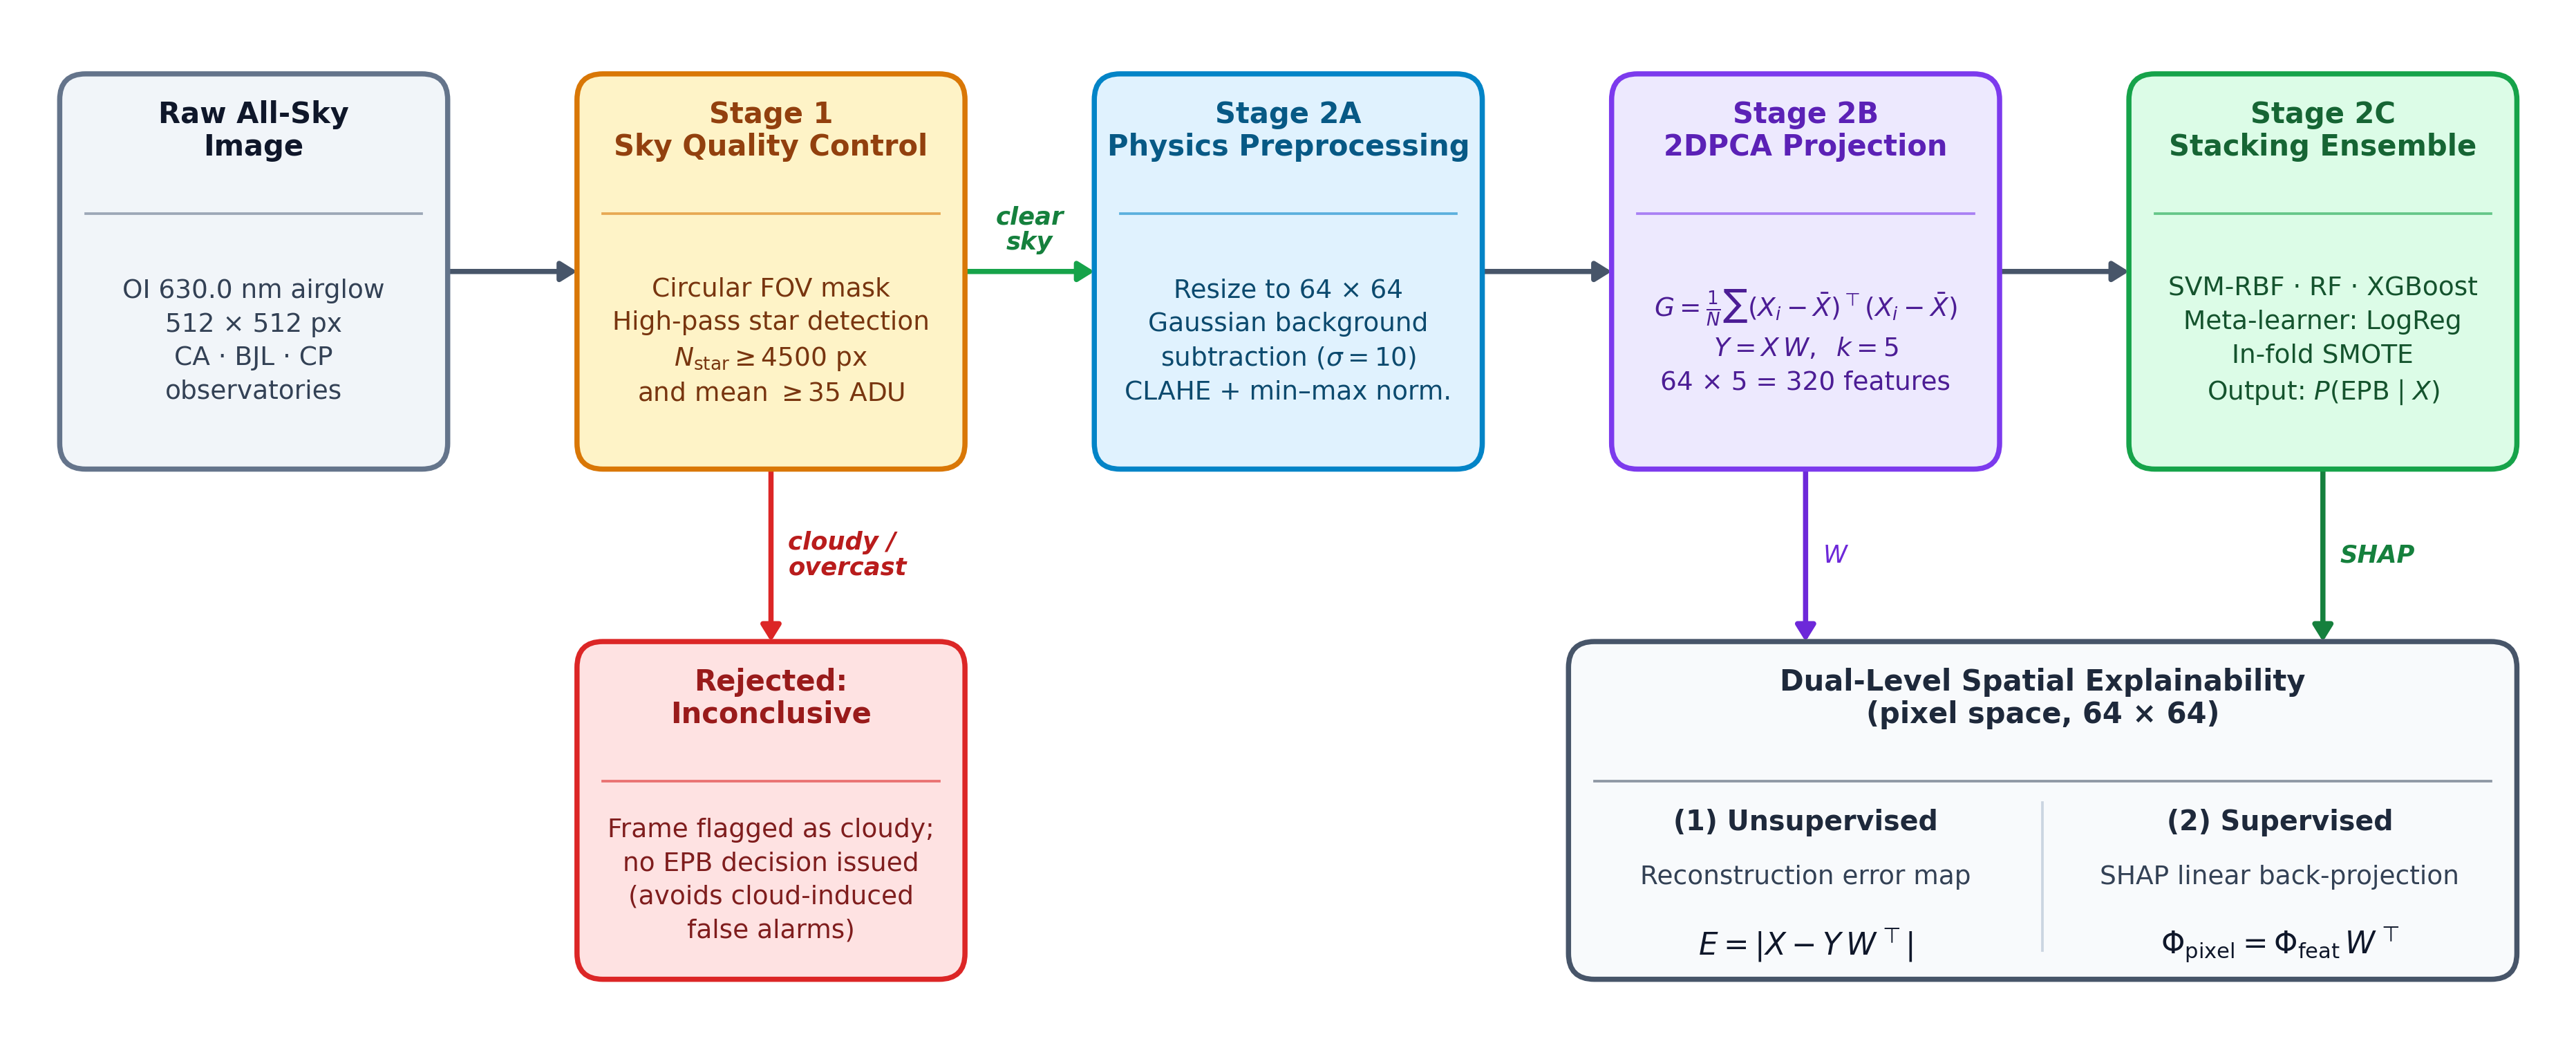
\includegraphics[width=0.98\textwidth]{figs/pipeline_architecture.png}
    \caption{Overview of the two-stage cascaded EPB detection pipeline. Stage~1 screens out cloud-contaminated exposures using star-pixel counts and mean luminance inside the circular field of view; Stage~2 applies background subtraction and CLAHE, extracts 2DPCA matrix features ($k=5$, $320$ features), and classifies frames with a stacking ensemble.}
    \label{fig:pipeline_arch}
\end{figure}

\subsection{Dataset}\label{sec:data}

The images come from the \textit{Estudo e Monitoramento Brasileiro do Clima Espacial} (EMBRACE) program of the Brazilian National Institute for Space Research (INPE). The instruments are all-sky CCD imagers with fish-eye lenses ($180^\circ$ field of view) and a narrow-band $630.0\text{ nm}$ filter. Each exposure is an $8$-bit $512 \times 512$ grayscale image, recorded every $3\text{--}5$ minutes.

\begin{table}[htbp]
\centering
\caption{Summary of the EMBRACE $630.0\text{ nm}$ all-sky dataset across observatories, lunar illumination regimes, and continuous nocturnal monitoring sequences.}
\label{tab:dataset}
\resizebox{\textwidth}{!}{%
\setlength{\tabcolsep}{5pt}
\begin{tabular}{llrrrr}
\toprule
\textbf{Dataset Subset / Observatory} & \textbf{Coordinates} & \textbf{Total} & \textbf{EPB} & \textbf{No-EPB} & \textbf{EPB (\%)} \\
\midrule
\multicolumn{6}{l}{\textit{Part A: Labeled Classification Dataset ($N = 572$ images, $16$ nights, $77$ temporal blocks)}} \\
São João do Cariri (CA) & $7.4^\circ\text{S}, 36.5^\circ\text{W}$ & 310 & 213 & 97 & 68.7\% \\
Bom Jesus da Lapa (BJL) & $13.3^\circ\text{S}, 43.4^\circ\text{W}$ & 220 & 0 & 220 & 0.0\% \\
Cachoeira Paulista (CP) & $22.7^\circ\text{S}, 45.0^\circ\text{W}$ & 42 & 42 & 0 & 100.0\% \\
\quad Low/Moderate Moon ($<50\%$) & All stations & 475 & 255 & 220 & 53.7\% \\
\quad Bright Lunar Glare ($\ge 50\%$) & All stations & 97 & 0 & 97 & 0.0\% \\
\textbf{Total Labeled Dataset} & \textbf{3 Stations} & \textbf{572} & \textbf{255} & \textbf{317} & \textbf{44.6\%} \\
\midrule
\multicolumn{6}{l}{\textit{Part B: Continuous Nocturnal Sequences ($986$ total frames across $8$ nights)}} \\
\texttt{BJL\_20250722} (Clear Quiet Sky) & $13.3^\circ\text{S}, 43.4^\circ\text{W}$ & 230 & 0 & 230 & 0.0\% \\
\texttt{CA\_20251022} (Active EPB Night) & $7.4^\circ\text{S}, 36.5^\circ\text{W}$ & 140 & 126 & 14 & 90.0\% \\
\texttt{CA\_20260624} (Overcast / Cloudy) & $7.4^\circ\text{S}, 36.5^\circ\text{W}$ & 62 & 0 & 62 & 0.0\% \\
Five Additional Monitoring Nights & CA / BJL / CP & 554 & -- & -- & Operational \\
\bottomrule
\end{tabular}%
}
\end{table}

The data are divided into two parts (Table~\ref{tab:dataset}). Part~A contains $572$ images labeled by an expert ($255$ with EPBs and $317$ without, a negative-to-positive ratio of $1.24:1$), taken on $16$ nights and grouped into $77$ non-overlapping $30$-minute windows. They come from three observatories at different magnetic latitudes: São João do Cariri (CA), Bom Jesus da Lapa (BJL), and Cachoeira Paulista (CP). The class balance differs a lot between sites, since BJL contributes only negative examples and CP only positive ones. A model that works on raw intensities could therefore separate the classes just by recognizing the station from its background brightness. Of the negatives from CA, $62$ were recorded under overcast skies. In addition, $97$ negatives ($17.0\%$ of Part~A) were taken with the Moon at least $50\%$ illuminated (fraction computed from each timestamp), when glare produces strong brightness gradients across the dome. Part~B has eight full-night sequences ($986$ frames), used to test temporal stability and cloud rejection.

\subsection{Stage 1: Sky Quality Control}\label{sec:stage1}

Clouds attenuate the $630.0\text{ nm}$ emission and create dark patches that, after contrast enhancement, look like plasma depletions. Stars give a simple measure of transparency: on a clear night many point sources are visible across the dome, while clouds blur or hide them.

Each raw $512 \times 512$ image $I_{\text{raw}}$, with values in $[0, 255]$, is restricted to a circular mask of radius $r = 0.44 \min(H, W)$ centered on the dome, which leaves out the station code and timestamp printed in the corners. To separate stars from the diffuse sky, we smooth the image with a Gaussian filter ($\sigma = 2.0$ pixels) and take the high-pass residual
\begin{equation}\label{eq:star_residual}
    R_{\text{high}}(x, y) = I_{\text{raw}}(x, y) - (G_{\sigma=2.0} * I_{\text{raw}})(x, y).
\end{equation}
A pixel $(x, y)$ inside the mask is counted as a star pixel if $R_{\text{high}}(x, y) > 8.0$ and $I_{\text{raw}}(x, y) > 30.0$, where the intensity threshold keeps dark-current noise in dark regions from being counted as stars. Let $N_{\text{star}}$ be the number of star pixels and $\mu_{\text{sky}}$ the mean of $I_{\text{raw}}$ inside the mask. A frame is labeled \texttt{CLOUDY} and discarded if $\mu_{\text{sky}} < 35.0$ or $N_{\text{star}} < 4500$. Frames with $4500 \le N_{\text{star}} < 6500$ go to Stage~2 with a partial-visibility flag (\texttt{DEGRADED}), and frames with $N_{\text{star}} \ge 6500$ go as \texttt{CLEAR}.

\subsection{Stage 2: Preprocessing, Augmentation, and Balancing}\label{sec:stage2}

Frames accepted by Stage~1 are resized to $64 \times 64$ pixels (bilinear interpolation), scaled to $[0, 1]$, and go through three steps meant to remove brightness variations that do not come from the ionosphere:
\begin{enumerate}
    \item Background subtraction: all-sky images show radial brightening toward the horizon (Van Rhijn effect) and smooth gradients from moonlight. We estimate this slowly varying component with a Gaussian filter ($\sigma = 10$ pixels) and subtract it, clipping negative values at zero: $I_{\text{sub}}(x,y) = \max\!\big(0,\, I(x,y) - (G_{\sigma=10} * I)(x,y)\big)$.
    \item Contrast equalization: Contrast Limited Adaptive Histogram Equalization (CLAHE, clip limit $0.03$) is applied to $I_{\text{sub}}$, so that faint depletion bands stand out without amplifying noise in uniform regions of the sky.
    \item Normalization and optional masking: the result is min-max normalized to $[0, 1]$, giving the input matrix $\mathbf{X} \in \mathbb{R}^{64 \times 64}$. To test the influence of the corner text, we also build a masked version $\mathbf{X}_{\text{mask}}$ in which all pixels outside $r = 0.44 \times 64$ are set to zero.
\end{enumerate}

The data are split before any augmentation, subspace fitting, or oversampling. Only training images are augmented, with transformations compatible with all-sky geometry: small rotations ($\pm 15^\circ$), horizontal flips, slight changes in brightness and contrast ($\pm 10\%$), and weak Gaussian noise ($\sigma = 0.02$). After 2DPCA extraction and z-score standardization (fitted on the training fold only), the Synthetic Minority Over-sampling Technique (SMOTE) \cite{chawla2002smote} balances the classes inside an \texttt{imblearn} pipeline, again on the training fold only. Validation and test sets are never augmented or resampled.

\subsection{2DPCA Projection, Stacking Ensemble, and Explainability}\label{sec:model}

Flattening a $64 \times 64$ image into a $4096$-dimensional vector loses the spatial neighborhood and requires estimating a $4096 \times 4096$ covariance matrix from a few hundred samples. 2DPCA \cite{yang2004two} instead computes a $64 \times 64$ image covariance matrix directly from the centered training matrices $\{\mathbf{X}_i \in \mathbb{R}^{64 \times 64}\}_{i=1}^{M}$ with sample mean $\bar{\mathbf{X}} = \frac{1}{M}\sum_{i=1}^{M} \mathbf{X}_i$:
\begin{equation}\label{eq:2dpca_cov}
    \mathbf{G} = \frac{1}{M}\sum_{i=1}^{M} (\mathbf{X}_i - \bar{\mathbf{X}})^\top (\mathbf{X}_i - \bar{\mathbf{X}}) \in \mathbb{R}^{64 \times 64}.
\end{equation}
Let $\mathbf{W} = [\mathbf{w}_1, \mathbf{w}_2, \dots, \mathbf{w}_k] \in \mathbb{R}^{64 \times k}$ contain the orthonormal eigenvectors of $\mathbf{G}$ associated with the $k$ largest eigenvalues $\lambda_1 \ge \lambda_2 \ge \dots \ge \lambda_k$. Projecting a centered image onto $\mathbf{W}$ yields the principal component matrix $\mathbf{Y}_i = (\mathbf{X}_i - \bar{\mathbf{X}})\mathbf{W} \in \mathbb{R}^{64 \times k}$. Each entry $Y_i(r, c)$, denoted as feature \texttt{PC\_Row\_$r$\_Comp\_$c$}, is the projection of image row $r \in \{0, \dots, 63\}$ onto the eigenvector $\mathbf{w}_c$ ($c \in \{0, \dots, k-1\}$); the row order is kept and only the horizontal variation is compressed. With $k=5$, chosen by cross-validation (Section~\ref{sec:kselect}), vectorizing $\mathbf{Y}_i$ gives a $320$-dimensional feature vector $\mathbf{z}_i$, $12.8$ times smaller than the image.

The standardized vector $\mathbf{z}_i$ is classified by a two-level stacking ensemble \cite{wolpert1992stacked} with three base learners:
\begin{enumerate}
    \item A Support Vector Machine (SVM) with a Radial Basis Function (RBF) kernel ($C = 5.0$, $\gamma = \text{scale}$, balanced class weights).
    \item An XGBoost classifier ($200$ trees, maximum depth $6$, learning rate $0.1$, subsample $0.8$, column subsample $0.8$).
    \item A Random Forest classifier ($200$ trees, maximum depth $15$, minimum leaf size $2$, balanced class weights).
\end{enumerate}
The out-of-fold probabilities of the three learners, obtained by an internal 5-fold cross-validation, are combined by an $\ell_2$-regularized Logistic Regression ($C = 1.0$).

To see where in the image the decisions come from, we use two maps. The first is unsupervised: reconstructing the image from its projection, $\hat{\mathbf{X}}_i = \bar{\mathbf{X}} + \mathbf{Y}_i \mathbf{W}^\top$, gives the error map $\mathbf{E}_i = |\mathbf{X}_i - \hat{\mathbf{X}}_i|$, which highlights local structures that the leading components do not capture. The second is supervised: we compute SHAP values \cite{lundberg2017unified} for the tree learners in the $320$-dimensional feature space, reshape them into $\boldsymbol{\Phi}_{\text{feat}} \in \mathbb{R}^{64 \times k}$, and, since 2DPCA is linear, map them back to pixels with $\boldsymbol{\Phi}_{\text{pixel}} = \boldsymbol{\Phi}_{\text{feat}}\mathbf{W}^\top$. Positive values mark pixels that raise the EPB probability, and negative values mark pixels that favor a quiet sky.

\subsection{Evaluation Protocol}\label{sec:protocol}

We report 5-fold stratified cross-validation on the $572$ labeled images and the results on a stratified holdout split with $25\%$ of the data ($n=143$). Because consecutive frames are correlated, we also run a 5-fold group cross-validation in which all frames of a $30$-minute window fall in the same fold (temporal-block CV), and we repeat the stratified CV on the masked inputs $\mathbf{X}_{\text{mask}}$ to check the effect of the corner text. Transfer between sites is measured by training on CA and BJL ($n=530$) and testing on CP ($n=42$) without any retraining (zero-shot). As CP has only EPB frames, this test measures recall only.

The pipeline is compared with classifiers on flattened pixels ($4096$ features) and on 1D-PCA ($320$ components), with each 2DPCA base learner used alone, and with a small 2D CNN ($\text{AvgPool}_{2\times 2} \to \text{Conv2D}_{8,5\times 5} \to \text{MaxPool}_{2\times 2} \to \text{Conv2D}_{16,3\times 3} \to \text{MaxPool}_{2\times 2} \to \text{Dense}_{32} \to \text{Sigmoid}$, trained for $25$ epochs with Adam). We also run three ablations: without radiometric preprocessing, without SMOTE, and with the circular mask. For the full-night tests with clouds, Stage~2 is retrained on the $510$ labeled images without cloud cover, so that no overcast frame is seen during training. We report accuracy, sensitivity (recall), specificity, precision, F1-score, ROC-AUC, PR-AUC, and CPU inference time per image.
